\section{Decomposition 1: SIoTIP System (Av3, UC14, UC15, UC18)}

\subsection{Module to decompose}
    In this run we decompose the \texttt{SIoTIP System}.


\subsection{Selected architectural drivers}
    The non-functional drivers for this decomposition are:
    \begin{itemize}
    	\item \emph{Av3}: Pluggable device or mote failure
    \end{itemize}

    \noindent The related functional drivers are:
    \begin{itemize}
    	\item \emph{UC14}: Send heartbeat (Av3) \\
              This use case checks whether or not motes and pluggable devices
              are still operational.
    	\item \emph{UC15}: Send notification (Av3) \\
              This use case sends a notification to a registered user.
    	\item \emph{UC18}: Check and deactivate applications (Av3) \\
              This use case deactivates any application that requires deactivation,
              because of unavailability of essential pluggable devices
              or unassigned mandatory roles.
    \end{itemize}

    \paragraph{Rationale}
        We chose Av3 first since it had high priority and it was more relevant to
        the core of the system (pluggable device data) than attributes M1 and U2. We
        chose P2 along with Av3 as it would force us to think about the way
        sensor data is handled. We believe this combination of pluggable device connectivity and
        storage of sensor data is the most defining feature of the system, and that
        handling this combination would give a better starting point than M1+U2
        for later ADD iterations.


\subsection{Architectural design}
    % Tactics:
    %     Detection:
    %         Ping/Echo
    %         Monitor
    %         Heartbeat
    %         Timestamp
    %     Resolution:
    %         notifications to 3 stakeholders
    %         degradation/removal from service -> turn off apps

    \paragraph{Application redundancy settings for Av3}
        Discussion of the solution selected for (a part of) one of the architectural
        drivers.

    \paragraph{Failure detection for Av3}
        timers? \\
        heartbeat/timestamp tactic

    \paragraph{Application deactivation for Av3}
        Applications need pluggable devices for the proper functioning. 
        When the pluggable devices fail, \texttt{the PluggableDeviceManager} sends 
        command and \texttt{the ApplicationManager} deactivate one or more applications 
        using those devices. Availability and reliability of the shared platform offered to applications is 
        important. To reduce the risk of frequent application downtime, 
        an application provider can require a redundancy in the available 
        pluggable devices. Multiple sensors or actuators for one application can be in one room.
        If one of sensor or actuator failed application just start using 
        the other available sensor or actuator in room. 

    \paragraph{Notifications for Av3}
        One of the important things for Av3 is notification. In the case 
        of failure of sensor, it is mandatory to inform all involved parties
         about the failure to resolve the problem as soon as possible. 
        \texttt{The NotificationHandler} notify an infrastructure owner of 
        any persistent pluggable device or mote failures. The infrastructure 
        owner has to receive the notification in ten seconds in case mote failed or 
        in thirty seconds if a pluggable device failed. Notification is also send 
        to a customer organisation, when one or more of their application are 
        susspended or re-activated. Applications using a failed  pluggable 
        device should be also notified via \texttt{The NotificationHandler}.

    \subsubsection{Alternatives considered}
        \paragraph{Alternatives for application deactivation for Av3}
            As mentioned above, when some of pluggable devices fail the applation can operate
            normally, because of using the next available sensor. ???? could be?


\subsection{Instantiation and allocation of functionality}
    \paragraph{Decomposition}
        Main aspects of the resulting decomposition.

        \begin{figure}[!htp]
        	\centering
        	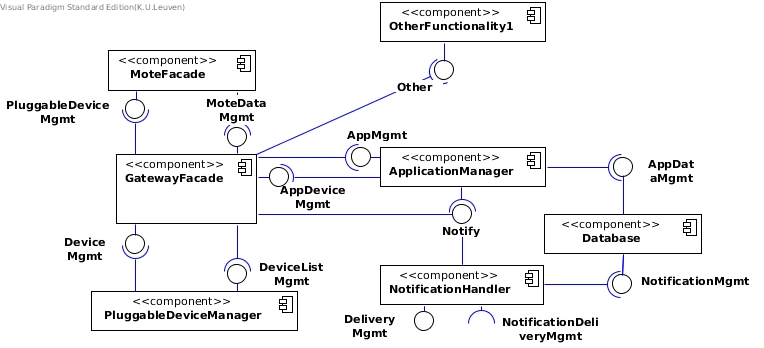
\includegraphics[width=1.00\textwidth]{component-diagram-1}
        	\caption{Component-and-connector diagram of this decomposition.}
            \label{fig:it1-cc_main}
        \end{figure}

    \subparagraph{ApplicationManager}
        Responsible for deactivating applications and after this action calls method of 
        \texttt{the NotificationHandler} to send notification to a customer organisation.
        When \texttt{the ApplicationManager} detects that application uses failed pluggable devices, 
        then the notification is sent to an application.

        set redundancy in the available pluggable devices??
        (Av3) ???? check mandatory user roles

    \subparagraph{Database}
        General database for other data. For instance the Database storages the data 
        of notifications (Av3).

    \subparagraph{GatewayFacade}
        Receives heartbeats from pluggable devices and sends heartbeats/device lists.
        \texttt{The GatewayFacade} sends commands to \texttt{the ApplicationManager}
        to shutdown applications, if is it needed. \\
        
        send notification trigger ???(Av3)\\
        forward data to applications

    \subparagraph{MoteFacade}
        Sends heartbeats from pluggable devices to\texttt{the PluggableDeviceFacade}.

    \subparagraph{NotificationHandler}
        Responsible for send notifications to infrastructure owner, customer organisation
        and applications (Av3). \\
        stored by system \(->\) contact DB? \\
        lookup communication channel \\
        users choose delivery method?

    \subparagraph{PluggableDeviceFacade}
        Sends heartbeats to \texttt{the MoteFacade}. 

    \subparagraph{PluggableDeviceManager}
        Checks list of devices and see if there are pluggable devices for applications.
        \texttt{the PluggableDeviceManager} contains application preferences (e.g. amount of sensors required) and 
        can send command to deactivate application.
        Send information about new/needed hardware is detected to \texttt{the GatewayFacade}, that sends command to
        reactivate application.
        check redundancy in the available pluggable devices??? is not the same like first sentence???

    % \paragraph{Behaviour}
    % If needed and explanation of the behaviour of certain aspects of the design so
    % far.
    % A SEQUENCE DIAGRAM FOR UC11 WOULD BE ACTUALLY VERY USEFUL (shows how the gateway checks if devices are initialised), 14 too: shows how applications can get deactivated
    % REMOVE THIS PART BECAUSE MONEYKA IS LAAAAZZZZYYYYYY BAD STUDENT "IT IS NOT NECESSARY"
    % \begin{figure}[!htp]
    % 	\centering
    % 	%\includegraphics[width=1.00\textwidth]{}
    % 	\missingfigure[figwidth=0.8\textwidth]{Sequence diagram}
    % 	\caption{Sequence diagram illustrating a key behavioural aspect.
    % 	}\label{fig:it1-seq_aspect1}
    % \end{figure}

    \paragraph{Deployment}
        Rationale of the allocation of components to physical nodes.

        \begin{figure}[!htp]
        	\centering
        	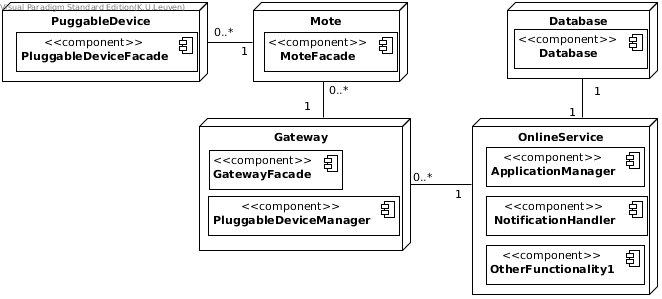
\includegraphics[width=1.00\textwidth]{deployment-diagram-1}
        	\caption{Deployment diagram of this decomposition.
        	}\label{fig:it1-depl_main}
        \end{figure}


\subsection{Interfaces for child modules}
    \subsubsection{ApplicationManager}
        \begin{itemize}
            \item ForwardData
            \begin{itemize}
                \item \texttt{void sendData(PluggableDeviceData data)}
                \begin{itemize}
                    \item Effect: Send pluggable device data to an application that wants to use it
                    \item Exceptions: None
                \end{itemize}
            \end{itemize}

            \item AppMgmt
            \begin{itemize}
                \item \texttt{void deactivateApplicationInstance(int applicationInstanceID)}
                \begin{itemize}
                    \item Effect: Deactivates a running instance of an application.
                    \item Exceptions: None
                \end{itemize}
                \item \texttt{void activateApplicationInstance(int applicationInstanceID)}
                \begin{itemize}
                    \item Effect: Activates a new instance of an application.
                    \item Exceptions: None
                \end{itemize}
            \end{itemize}
        \end{itemize}

    \subsubsection{Database}
        \begin{itemize}
            \item NotificationMgmt
            \begin{itemize}
                \item \texttt{int storeNotification(NotificationData data)}
                \begin{itemize}
                    \item Effect: Stores a new notification entry in the database. Returns the id of the new notification.
                    \item Exceptions: None
                \end{itemize}
                \item \texttt{void updateNotification(NotificationData data)}
                \begin{itemize}
                    \item Effect: Updates an existing notification (e.g. change status to "sent").
                    \item Exceptions: None
                \end{itemize}
                \item \texttt{int lookupNotificationChannelForUser(int userID)}
                \begin{itemize}
                    \item Effect: Returns the type of communication channel a user prefers.
                                  Different communication channels are mapped to integers.
                    \item Exceptions: None
                \end{itemize}
            \end{itemize}

            \item AppDataMgmt
            \begin{itemize}
                \item \texttt{void updateApplication(ApplicationData data)}
                \begin{itemize}
                    \item Effect: Updates an application in the database (e.g. change state to 'inactive').
                    \item Exceptions: None
                \end{itemize}
                \item \texttt{void updateSubscription(SubscriptionData data)}
                \begin{itemize}
                    \item Effect: Updates a subscription in the database (e.g. change state to 'disabled').
                    \item Exceptions: None
                \end{itemize}
            \end{itemize}
        \end{itemize}

    \subsubsection{GatewayFacade}\label{add1-int-gatewayfacade}
        \begin{itemize}
            \item MoteDataMgmt
            \begin{itemize}
                \item \texttt{void sendHeartbeat(int moteID, List<PluggableDeviceInfo> devices)}
                \begin{itemize}
                    \item Effect: Sends a heartbeat to a certain gateway with information about operational devices.
                    \item Exceptions: None
                \end{itemize}
            \end{itemize}

            \item DeviceMgmt
            \begin{itemize}
                \item \texttt{List<DeviceInfo> getConnectedDevices()}
                \begin{itemize}
                    \item Effect: Describe the effect of calling this operation.
                    \item Exceptions: None
                \end{itemize}
                \item \texttt{void timerExpired(int deviceID)}
                \begin{itemize}
                    \item Effect: Lets the gateway know that a timer for pluggable device or mote has expired.
                                  This will generate a notification for an infrastructure owner.
                    \item Exceptions: None
                \end{itemize}
                \item \texttt{void deactivateApplicationInstance(int applicationInstanceID)}
                \begin{itemize}
                    \item Effect: Deactivates a certain application. This could happen when
                                  mandatory pluggable devices for the application are missing.
                    \item Exceptions: None
                \end{itemize}
                \item \texttt{void reactivateApplicationInstance(int applicationInstanceID)}
                \begin{itemize}
                    \item Effect: Reactivate an application instance. This could happen
                                  automatically after a broken sensor has been replaced.
                    \item Exceptions: None
                \end{itemize}
            \end{itemize}

            \item AppDeviceMgmt
            \begin{itemize}
                \item \texttt{bool areEssentialDevicesOperational(int applicationID)}
                \begin{itemize}
                    \item Effect: Returns true if all essential devices for the application
                                  with id "applicationID" are operational.
                    \item Exceptions: None
                \end{itemize}
            \end{itemize}
        \end{itemize}

    \subsubsection{MoteFacade}\label{add1-int-motefacade}
        \begin{itemize}
            \item PluggableDeviceDataMgmt
            \begin{itemize}
                \item \texttt{List<DeviceInfo> getConnectedDevices()}
                \begin{itemize}
                    \item Effect: Returns a list of information about devices that are connected to the mote.
                    \item Exceptions: None
                \end{itemize}
            \end{itemize}
        \end{itemize}

    \subsubsection{NotificationHandler}
        \begin{itemize}
            \item Notify
            \begin{itemize}
                \item \texttt{void notify(int userID, String message)}
                \begin{itemize}
                    \item Effect: Describe the effect of calling this operation.
                    \item Exceptions: None
                \end{itemize}
            \end{itemize}

            \item DeliveryMgmt
            \begin{itemize}
                \item \texttt{void sendAcknowledgement(int notificationID)}
                \begin{itemize}
                    \item Effect: Sends an acknowledgement to the system for a certain notification.
                    \item Exceptions: None
                \end{itemize}
            \end{itemize}
        \end{itemize}

    \subsubsection{External notification delivery serivce}
        \begin{itemize}
            \item NotificationDeliveryMgmt
            \begin{itemize}
                \item \texttt{void notify(JSONObject data)}
                \begin{itemize}
                    \item Effect: Deliver a notification to an end user using a specific delivery service.
                    \item Exceptions: None
                \end{itemize}
            \end{itemize}
        \end{itemize}

    \subsubsection{PluggableDeviceManager}
        \begin{itemize}
        	\item DeviceListMgmt
        	\begin{itemize}
        		\item \texttt{void sendHeartbeat(int moteID, List<PluggableDeviceInfo> devices)}
        		\begin{itemize}
        			\item Effect: Send a heartbeat from a mote to check/update timers for operational devices.
        			\item Exceptions: None
        		\end{itemize}
        		\item \texttt{bool areEssentialDevicesOperational(int applicationID)}
        		\begin{itemize}
        			\item Effect: Returns true if all essential devices for the application
                                  with id "applicationID" are operational.
        			\item Exceptions: None
        		\end{itemize}
        	\end{itemize}
        \end{itemize}


\subsection{Data type definitions}
    \paragraph{PluggableDeviceData}
              contains data from a pluggable device at a certain point in time
              (value, type, date) (e.g. a sensor reading, an actuator status)
    \paragraph{PluggableDeviceSettings}
              contains settings for a pluggable device (power status,
              data update rate, ...)
    \paragraph{PluggableDeviceInfo}
              contains information about a pluggable device (device id,
              power status, data update rate, ...)

    \paragraph{NotificationData}
              contains data about a notification (message text, recipient,
              communication channel, date, status, source, ...).

    \paragraph{ApplicationData}
              contains data about an application instance (instance id, running status, ...)
    \paragraph{SubscriptionData}
              contains data about a subscription (subscription id, subscription status,
              subscription period, ...).


\subsection{Verify and refine}
    Completely handled: Av3, UC14, UC15, UC18 \\

    \noindent This section describes per component which (parts of) the remaining
    requirements it is responsible for.

    \paragraph{ApplicationManager}
        \begin{itemize}
            \item  \emph{Av2}: Application failure \\
                   Prevention: a, b \\
                   Detection: a, b, c \\
                   Resolution: a, b, c
           \item \emph{P1}: Large number of users: c
           \item \emph{M1}: Integrate new sensor or actuator manufacturer: 1.c, 2.a
           \item \emph{M2}: Big data analytics on pluggable data and/or application usage data: d, e
           \item \emph{U1}: Application updates: a, b, c, d
           \item \emph{U2}: Easy Installation: e
           \item \emph{U12}: Perform actuation command
           \item \emph{UC17}: Activate an application: 3, 4
        \end{itemize}

    \paragraph{Database}
        \begin{itemize}
          	\item None
        \end{itemize}

    \paragraph{GatewayFacade}
        \begin{itemize}
            \item \emph{Av1}: Communication between SIoTIP gateway and Online Service \\
                               Resolution: b, c, d
            \item \emph{M1}: Integrate new sensor or actuator manufacturer: 1.a, 2.b
            \item \emph{U2}: Easy Installation: a, c, d
            \item \emph{UC11}: Send pluggable device data: 1
        \end{itemize}

    \paragraph{MoteFacade}
        \begin{itemize}
            \item \emph{M1}: Integrate new sensor or actuator manufacturer: 1.a, 2.b
            \item \emph{U2}: Easy Installation: b, c, d
            \item \emph{UC4}: Install mote: 1, 2
            \item \emph{UC5}: Uninstall mote: 1
            \item \emph{UC6}: Insert a pluggable device into a mote: 2
            \item \emph{UC7}: Remove a pluggable device from its mote: 2
            \item \emph{UC11}: Send pluggable device data: 1
        \end{itemize}

    \paragraph{NotificationHandler}
        \begin{itemize}
            \item \emph{UC16}: Consult notification message: 5
            \item \emph{UC17}: Activate an application: 5, 6
        \end{itemize}

    \paragraph{OtherFunctionality}
        \begin{itemize}
            \item \emph{Av1}: Communication between SIoTIP gateway and Online Service \\
                               Detection: a, b, c, d
                               Resolution: a
           	\item \emph{P1}: Large number of users: a
            \item \emph{P2}: Requests to the pluggable data database
            \item \emph{M1}: Integrate new sensor or actuator manufacturer: 1.d
            \item \emph{M2}: Big data analytics on pluggable data and/or application usage data: a
            \item \emph{U2}: Easy Installation: e
            \item \emph{UC1}: Register a customer organisation
            \item \emph{UC2}: Register an end-user
            \item \emph{UC3}: Unregister an end user
            \item \emph{UC4}: Install mote: 3
            \item \emph{UC5}: Uninstall mote: 2.b
            \item \emph{UC6}: Insert a pluggable device into a mote: 3: topology part; alternative 3a.1.b
            \item \emph{UC7}: Remove a pluggable device from its mote: 3.b
            \item \emph{UC8}: Initialise a pluggable device: 1, 2, 4
            \item \emph{UC9}: Configure pluggable device access rights
            \item \emph{UC10}: Consult and configure the topology
            \item \emph{UC11}: Send pluggable device data: 3
            \item \emph{UC13}: Configure pluggable device
            \item \emph{UC16}: Consult notification message: 1, 2, 3, 4
            \item \emph{UC17}: Activate an application: 1, 2
            \item \emph{UC19}: Subscribe to application
            \item \emph{UC20}: Unsubscribe from application
            \item \emph{UC21}: Send invoice
            \item \emph{UC22}: Upload an application
            \item \emph{UC23}: Consult application statistics
            \item \emph{UC24}: Consult historical data
            \item \emph{UC25}: Access topology and available devices
            \item \emph{UC26}: Send application command or message to external front-end
            \item \emph{UC27}: Receive application command or message to external front-end
            \item \emph{UC28}: Log in
            \item \emph{UC29}: Log out
        \end{itemize}

    \paragraph{PluggableDeviceDB}
        \begin{itemize}
            \item \emph{M1}: Integrate new sensor or actuator manufacturer: 1.a, 1.b, 2.b
            \item \emph{M2}: Big data analytics on pluggable data and/or application usage data: b
        \end{itemize}

    \paragraph{PluggableDeviceFacade}
        \begin{itemize}
        	\item \emph{U2}: Easy Installation: d
        \end{itemize}

    \paragraph{PluggableDeviceManager}
        \begin{itemize}
            \item \emph{U2}: Easy Installation: c, d
            \item \emph{UC4}: Install mote: 4
            \item \emph{UC5}: Uninstall mote: 2
            \item \emph{UC6}: Insert a pluggable device into a mote: 3: uninitialised part; alternative 3a.1 3a.2 3a.4; 4
            \item \emph{UC7}: Remove a pluggable device from its mote: 3.a, 3.c
            \item \emph{UC8}: Initialise a pluggable device: 3
            \item \emph{UC11}: Send pluggable device data: 2, 3a
        \end{itemize}

    \paragraph{PluggableDeviceDataScheduler}
        \begin{itemize}
            \item \emph{P1}: Large number of users: b
            \item \emph{M1}: Integrate new sensor or actuator manufacturer: 1.a, 2.b
            \item \emph{M2}: Big data analytics on pluggable data and/or application usage data: b, c
        \end{itemize}
